% ADD TO THESE COMMENTS AS YOU SEE FIT 
%
% Testing - Internal Testing, give to the supervisors for feedback, changed according to their requirements
% CORRECT PRIMER PAIR
% Select from 155 to 1091.
% Forward: agagaagttctctcgacgcag
% Reverse: cctgtattctgttcccggttt
% Demo - dry run through with students. Given user guide and feedback sheets, changed according to their feedback
%
% Questionnaire - Sent out with jar file on moodle, feedback from students on 'finished' application

As with any software development, testing is a necessary component. During our time with the PCR application, testing begun
almost as soon as implementation started. Our testing fell into two categories:

\begin{itemize}
\item Testing of the backend, such as primer checking formulas etc.
\item Testing of the user interface.
\end{itemize}

Also, with reference to the (edit ME)\cite{Lethbridge}, we
accommodated for both white and black box testing. Our testing had to
ensure that the program met the requirements of the clients, which
were gathered in our several meetings with them.

\subsection{Methods Of Testing}
\subsubsection{White Box Testing}
White box testing was used throughout the development of the
implementation, as we all had an in-depth knowledge of the source
code. 
This enabled us to test for defects and errors by creating
scenarios which tested the programs to its limits and beyond, in order
for us to assure our code could be used to check primers
appropriately. 
We had a default DNA sequence that we used to conduct white box
testing, see see figure \ref{fig:demoBuild:test}.
In this sequence, we knew we had good primers to test the system, and
also bad primers to test the systems error checking. 
Due to the nature of white box testing, we were able to change the
implementation when we came across errors quickly and efficiently as
we knew what part of the code was failing by the nature of the error.
It also allowed for us to deliberately try to break the program to
ensure that when it error handled it did so in a safe and correct
manner, and didn't crash on the user.
%
%\begin{figure}[h]
%  \begin{center}
%    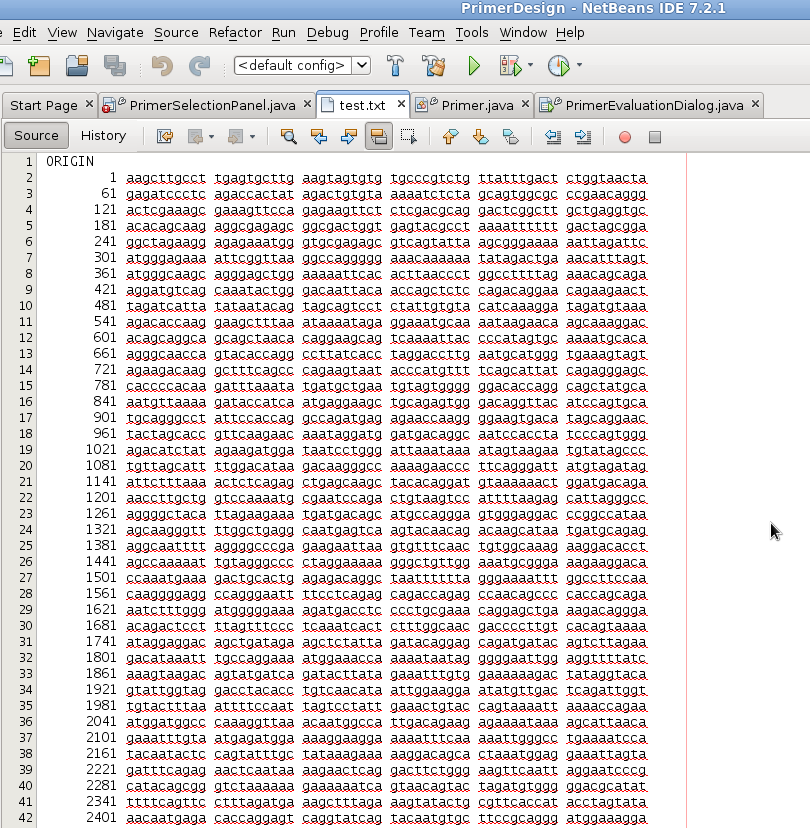
\includegraphics[width=0.9\textwidth]{./images/demoBuild/test.png}
%    \caption{
%      \label{fig:demoBuild:test}
%      Test.txt, a sample DNA sequence
%    }
%  \end{center}
%\end{figure}

\subsubsection{Black Box Testing}

Another important testing method we implemented was black box testing,
which allowed users with no knowledge of the implementation to test
our program for errors and defects.
This was done by our Demo test done on the 8th February 2013, (See:
Demonstration).
This was also carried out by users when we uploaded the final
implementation on moodle, using their feedback from their experiences
with it (See: Questionnaire).
This method of testing allowed us to gain new insights into what the
program does well and what it doesn't, and allowed us to make further
changes ontop of the changes already made thanks to our white box
testing.

\newpage




